% ============================================================================
% Mục 4.1 - Người viết: B
% ============================================================================
\subsection{Xây dựng đặc trưng (Phần B)}\label{sec:features}

Mục này mô tả mô-đun \code{src/features.py}: từ ba tập train/val/test do phần A tạo ra, sinh ra
\textbf{39 đặc trưng} thuộc ba nhóm --- \emph{lịch}, \emph{độ trễ (lag)} và \emph{thời tiết} --- dùng chung
cho mọi mô hình của nhóm (C, D). Mục tiêu thiết kế là: (i) mỗi đặc trưng đều phải \emph{quan sát được tại
thời điểm phát hành dự báo}; (ii) có cơ sở miền (domain) rõ ràng; (iii) tái lập được và có kiểm thử tự động.

\subsubsection{Thiết lập bài toán và nguyên tắc chống rò rỉ}\label{sec:setup}

\paragraph{Chân trời dự báo.} Phần B chọn \textbf{dự báo trước một ngày} ($h=24$ giờ) làm bài toán chính,
vì đây là thiết lập thực tế của thị trường điện ngày tới (OMIE) và của đơn vị vận hành lưới (REE). Chân trời
được tham số hóa qua \code{FeatureConfig(horizon=h)}; \cref{sec:horizon} so sánh thêm $h=1$.

\paragraph{Nguyên tắc chống rò rỉ (data leakage).} Mọi đặc trưng tại hàng $t$ được xây dựng sao cho:
\begin{enumerate}
  \item \textbf{Độ trễ $\geq h$}: chỉ dùng $y_{t-k}$ với $k\geq h$. Với $h=24$, các độ trễ 1--3 giờ bị
        loại bỏ tự động (\code{effective_lags}) dù có trong cấu hình.
  \item \textbf{Cửa sổ trượt kết thúc tại $t-h$}: thống kê trượt (trung bình, độ lệch chuẩn, min, max)
        được tính trên chuỗi đã dịch $y_{t-h}$, không bao giờ chứa $y_t$.
  \item \textbf{Tính trên trục thời gian liên tục}: ba tập được nối theo thứ tự thời gian, tính đặc trưng,
        rồi cắt lại theo mốc thời gian của phần A. Nhờ vậy 336 giờ đầu của tập validation vẫn có đặc trưng
        lag (lấy từ cuối tập train --- là quá khứ hợp lệ) và \textbf{không mất dòng nào} của val/test; chỉ
        672 giờ (4 tuần) đầu của tập train bị loại do chưa đủ lịch sử.
  \item \textbf{Loại các cột không có tại thời điểm dự báo}: các cột sản lượng phát (\code{generation *}),
        giá (\code{price actual}) phản ánh chính phụ tải giờ $t$; cột \code{total load forecast} là dự báo
        của TSO (tương quan 0.99 với mục tiêu, \cref{fig:eda}). Các cột này \emph{không bao giờ} là đầu vào;
        riêng \code{total load forecast} chỉ dùng làm mốc tham chiếu (\cref{sec:baselines}).
  \item \textbf{Chuẩn hóa nằm trong pipeline mô hình}: \code{StandardScaler} chỉ được \code{fit} trên tập
        huấn luyện của từng lần fit (\cref{sec:linear}), không chuẩn hóa trước trên toàn bộ dữ liệu.
\end{enumerate}

\paragraph{Giả định về thời tiết.} Đặc trưng thời tiết tại giờ $t$ sử dụng giá trị \emph{quan sát} tại $t$,
tương đương giả định có dự báo thời tiết hoàn hảo cho ngày mai. Đây là giả định phổ biến trong nghiên cứu
STLF~\cite{hong2016probabilistic}; trong vận hành thực tế, sai số dự báo nhiệt độ sẽ làm sai số phụ tải tăng nhẹ.

\subsubsection{Nhóm 1 -- Đặc trưng lịch (15 đặc trưng)}\label{sec:feat-cal}

Dữ liệu gốc lưu thời gian theo UTC, và phần A trích \code{hour}, \code{dayofweek} theo UTC. Tuy nhiên hành vi
tiêu dùng điện bám theo \textbf{giờ địa phương}: Tây Ban Nha dùng CET (UTC+1) vào mùa đông và CEST (UTC+2) vào
mùa hè. Nếu dùng giờ UTC, đỉnh phụ tải buổi sáng sẽ ``trượt'' một giờ giữa hai mùa. Phần B vì vậy chuyển
sang múi giờ \code{Europe/Madrid} trước khi trích đặc trưng (\cref{lst:calendar}).

\begin{table}[H]
\centering
\caption{Đặc trưng lịch (tiền tố \code{cal_}).}\label{tab:feat-cal}
\small
\begin{tabularx}{\linewidth}{lX}
\toprule
Đặc trưng & Ý nghĩa\\
\midrule
\code{hour}, \code{dayofweek}, \code{month}, \code{dayofyear} & Giờ (0--23), thứ (0 = Thứ Hai), tháng, ngày trong năm, theo giờ địa phương.\\
\code{is_weekend} & 1 nếu Thứ Bảy/Chủ Nhật.\\
\code{is_holiday} & 1 nếu là ngày lễ quốc gia Tây Ban Nha (1/1, 6/1, Thứ Sáu Tuần Thánh, 1/5, 15/8, 12/10, 1/11, 6/12, 8/12, 25/12).\\
\code{is_offday} & Cuối tuần \emph{hoặc} ngày lễ --- ngày nghỉ nói chung.\\
\code{is_bridge} & Ngày ``cầu'' (\emph{puente}): ngày làm việc kẹp giữa hai ngày nghỉ, nhiều người nghỉ phép.\\
\code{is_dst} & 1 khi áp dụng giờ mùa hè (CEST); tính từ độ lệch giờ địa phương -- UTC.\\
\code{hour_sin/cos}, \code{dow_sin/cos}, \code{doy_sin/cos} & Mã hóa tuần hoàn $\sin(2\pi x/P)$, $\cos(2\pi x/P)$ với chu kỳ $P = 24, 7, 365.25$.\\
\bottomrule
\end{tabularx}
\end{table}

\paragraph{Tại sao cần mã hóa tuần hoàn?} Biến giờ dạng số nguyên coi 23h và 0h cách nhau 23 đơn vị, trong
khi thực tế chúng liền kề. Ánh xạ lên đường tròn đơn vị,
\begin{equation}
  x \mapsto \bigl(\sin(2\pi x/P),\ \cos(2\pi x/P)\bigr),
\end{equation}
bảo toàn khoảng cách tuần hoàn. Mô hình tuyến tính hưởng lợi nhiều nhất; mô hình cây vẫn dùng được cả hai
dạng. Với mô hình tuyến tính, ngoài dạng tuần hoàn, \code{hour}, \code{dayofweek}, \code{month} còn được
mã hóa one-hot và thêm tương tác \code{hour}~$\times$~\code{is_offday} (\cref{sec:linear}).

\begin{lstlisting}[caption={Trích đặc trưng lịch theo giờ địa phương (rút gọn từ \code{features.py}).},label={lst:calendar}]
local = df["time"].dt.tz_convert("Europe/Madrid")
local_date = local.dt.tz_localize(None).dt.normalize()
hour, dow = local.dt.hour, local.dt.day_of_week
is_holiday = local_date.isin(SPAIN_HOLIDAYS)
out["cal_is_offday"] = ((dow >= 5) | is_holiday).astype(int)
utc_offset = local.dt.tz_localize(None) - df["time"].dt.tz_localize(None)
out["cal_is_dst"] = (utc_offset == pd.Timedelta(hours=2)).astype(int)  # CEST
out["cal_hour_sin"] = np.sin(2 * np.pi * hour / 24)
\end{lstlisting}

\subsubsection{Nhóm 2 -- Đặc trưng độ trễ và cửa sổ trượt (13 đặc trưng)}\label{sec:feat-lag}

Phụ tải điện có quán tính và tính mùa vụ theo ngày/tuần, nên giá trị quá khứ là đặc trưng mạnh nhất. Với
$h=24$, tập độ trễ hiệu lực là $\{24, 48, 72, 168, 336\}$ giờ:

\begin{table}[H]
\centering
\caption{Đặc trưng độ trễ (với $h=24$). Ký hiệu $\tilde{y}_t = y_{t-h}$ là giá trị gần nhất quan sát được.}\label{tab:feat-lag}
\small
\begin{tabularx}{\linewidth}{lX}
\toprule
Đặc trưng & Công thức / Ý nghĩa\\
\midrule
\code{lag_24}, \code{lag_48}, \code{lag_72} & $y_{t-24}, y_{t-48}, y_{t-72}$: cùng giờ 1, 2, 3 ngày trước.\\
\code{lag_168}, \code{lag_336} & $y_{t-168}, y_{t-336}$: cùng giờ, cùng thứ 1 và 2 tuần trước.\\
\code{roll_mean_24}, \code{roll_std_24} & Trung bình, độ lệch chuẩn của $\tilde{y}$ trong 24 giờ: mức nền và biên độ của ngày gần nhất.\\
\code{roll_mean_168}, \code{roll_std_168} & Như trên với cửa sổ 1 tuần: mức nền theo tuần.\\
\code{roll_min_24}, \code{roll_max_24} & Đáy đêm và đỉnh ngày của ngày gần nhất.\\
\code{lag_same_hour_4w_mean} & $\frac14\sum_{k=1}^{4} y_{t-168k}$: trung bình cùng giờ cùng thứ của 4 tuần trước.\\
\code{diff_24} & $y_{t-24} - y_{t-48}$: xu hướng tăng/giảm giữa hai ngày gần nhất.\\
\bottomrule
\end{tabularx}
\end{table}

\begin{lstlisting}[caption={Đặc trưng độ trễ luôn dịch ít nhất $h$ giờ.},label={lst:lags}]
y = df[TARGET]
for lag in cfg.effective_lags:            # only lags >= horizon
    out[f"lag_{lag}"] = y.shift(lag)
base = y.shift(cfg.horizon)                # last observable value
for w in cfg.roll_windows:                 # (24, 168)
    out[f"roll_mean_{w}"] = base.rolling(w, min_periods=w).mean()
    out[f"roll_std_{w}"]  = base.rolling(w, min_periods=w).std()
\end{lstlisting}

\subsubsection{Nhóm 3 -- Đặc trưng thời tiết (11 đặc trưng)}\label{sec:feat-weather}

EDA của phần A (\cref{fig:eda}, ô 2) cho thấy quan hệ nhiệt độ--phụ tải có dạng \textbf{chữ U}: phụ tải tăng
khi trời lạnh (sưởi) và khi trời nóng (điều hòa), thấp nhất quanh 15--19\,°C. Một hệ số tuyến tính duy nhất
cho nhiệt độ không thể biểu diễn quan hệ này, nên phần B xây dựng các biến đổi phi tuyến dựa trên khái niệm
\emph{độ-giờ sưởi/làm mát} (heating/cooling degree hours) quen thuộc trong ngành năng lượng:
\begin{align}
  \mathrm{HDH}_t &= \max\bigl(0,\ T_{\text{base}} - T_t\bigr), \qquad T_{\text{base}} = 18\,^\circ\mathrm{C},\\
  \mathrm{CDH}_t &= \max\bigl(0,\ T_t - (T_{\text{base}} + 4)\bigr),
\end{align}
trong đó $T_t$ là nhiệt độ trung bình 5 thành phố (đổi từ Kelvin sang °C). Khoảng 18--22\,°C là ``vùng thoải
mái'' không cần sưởi hay làm mát.

\begin{table}[H]
\centering
\caption{Đặc trưng thời tiết (tiền tố \code{w_}).}\label{tab:feat-weather}
\small
\begin{tabularx}{\linewidth}{lX}
\toprule
Đặc trưng & Ý nghĩa\\
\midrule
\code{temp_c} & Nhiệt độ trung bình (°C).\\
\code{temp_c_sq} & $(T_t - 18)^2$: thành phần bậc hai mô tả dạng chữ U.\\
\code{hdh}, \code{cdh} & Độ-giờ sưởi và làm mát (hàm hinge, tuyến tính từng khúc).\\
\code{temp_range} & $T_{\max} - T_{\min}$ giữa các thành phố: mức độ chênh lệch nhiệt vùng miền.\\
\code{humidity}, \code{pressure}, \code{wind_speed}, \code{clouds} & Độ ẩm, áp suất, gió, mây (trung bình 5 thành phố).\\
\code{temp_roll24} & Nhiệt độ trung bình 24 giờ qua: \emph{quán tính nhiệt} của tòa nhà.\\
\code{temp_roll24_diff} & $T_t - \overline{T}_{24h}$: thay đổi nhiệt đột ngột so với ngày trước.\\
\bottomrule
\end{tabularx}
\end{table}

\paragraph{Lưu ý về \code{temp_dev_mean} của phần A.} Cột này được tính bằng cách trừ nhiệt độ trung bình
của từng thành phố trên \emph{toàn bộ} 4 năm, tức có dùng thông tin của tập test. Phần B không dùng cột này để
tránh rò rỉ (dù mức độ rò rỉ nhỏ, chỉ là một hằng số theo thành phố).

\subsubsection{Kiểm thử tự động}\label{sec:feat-tests}

File \code{tests/test_features_and_evaluate.py} bổ sung các kiểm thử cho phần B:
\begin{itemize}
  \item \textbf{Không nhìn trước tương lai}: trên một chuỗi tổng hợp $y_t = t + c$, kiểm tra
        \code{lag_k}$\,= y_t - k$, cửa sổ trượt kết thúc đúng tại $t-h$ và không đặc trưng lag nào
        $\geq y_t$, với cả $h=1$ và $h=24$.
  \item \textbf{Múi giờ và ngày lễ}: 08:00 UTC ngày 1/1/2018 phải là 9h địa phương và là ngày lễ;
        22:30 UTC ngày 15/7/2018 phải là 0h ngày 16/7 (Thứ Hai) trong giờ mùa hè.
  \item \textbf{Trên dữ liệu thật}: val/test giữ đủ 5\,260 dòng, không còn NaN, các tập không chồng lấn.
  \item Mục tiêu, dự báo TSO và cột thời gian không lọt vào danh sách đặc trưng.
\end{itemize}

% Kết quả thực nghiệm của phần B (chạy bằng src/train_models.py)
\subsubsection{Đánh giá đóng góp của từng nhóm đặc trưng (ablation)}\label{sec:ablation}

Để kiểm chứng các nhóm đặc trưng có thực sự hữu ích, phần B huấn luyện Random Forest (100 cây, siêu tham số tốt
nhất ở \cref{sec:rf}) và Ridge ($\alpha=1$) trên tập train với từng tổ hợp nhóm đặc trưng, rồi đo trên tập
validation ($h=24$).

\begin{table}[H]
\centering
\caption{Ablation nhóm đặc trưng -- sai số trên tập validation ($h=24$). In đậm: tốt nhất mỗi cột.}\label{tab:ablation}
\small
\setlength{\tabcolsep}{5pt}
\begin{tabular}{lrrrrr}
\toprule
& & \multicolumn{2}{c}{Random Forest} & \multicolumn{2}{c}{Ridge}\\
\cmidrule(lr){3-4}\cmidrule(lr){5-6}
Nhóm đặc trưng & Số ĐT & MAE (MW) & MAPE (\%) & MAE (MW) & MAPE (\%)\\
\midrule
Chỉ thời tiết & 11 & 3\,370 & 11.63 & 3\,507 & 12.12\\
Chỉ lag & 13 & 1\,825 & 6.36 & 2\,012 & 7.03\\
Chỉ lịch & 15 & 1\,798 & 6.06 & 2\,064 & 7.04\\
Lag + thời tiết & 24 & 1\,875 & 6.51 & 2\,024 & 7.04\\
Lịch + thời tiết & 26 & 1\,736 & 5.91 & 2\,074 & 7.07\\
Lịch + lag & 28 & 1\,545 & 5.29 & \textbf{1\,852} & \textbf{6.39}\\
\textbf{Tất cả (3 nhóm)} & 39 & \textbf{1\,536} & \textbf{5.28} & 1\,870 & 6.44\\
\bottomrule
\end{tabular}
\end{table}

\paragraph{Nhận xét.}
\begin{itemize}
  \item \textbf{Lịch và lag bổ trợ cho nhau}: mỗi nhóm riêng lẻ cho MAE khoảng 1\,800~MW, nhưng kết hợp thì
        giảm còn 1\,545~MW ($-14\%$). Lag cho biết \emph{mức} phụ tải gần đây; lịch cho biết \emph{hình dạng}
        trong ngày và ngày nghỉ --- điều mà lag 24 giờ không biết (ví dụ dự báo cho Thứ Hai bằng dữ liệu Chủ Nhật).
  \item \textbf{Thời tiết đứng riêng rất yếu} (MAPE 11.6\%) vì không biết giờ trong ngày, nhưng thêm vào
        lịch thì vẫn giảm MAE từ 1\,798 xuống 1\,736~MW với Random Forest. Khi đã có lag, phần lớn thông tin
        thời tiết đã ``nằm sẵn'' trong phụ tải hôm qua (nhiệt độ thay đổi chậm), nên đóng góp biên chỉ còn
        $\approx 9$~MW.
  \item \textbf{Với Ridge, thêm thời tiết làm tệ đi nhẹ} (1\,852 $\to$ 1\,870~MW): quan hệ nhiệt độ--phụ tải
        phụ thuộc giờ trong ngày (\cref{fig:eda}, ô 2) mà mô hình tuyến tính cộng tính không biểu diễn được,
        nên các biến thời tiết chủ yếu thêm nhiễu. Đây là một lý do mô hình cây vượt trội ở \cref{sec:compare-c}.
\end{itemize}
Bộ đặc trưng đầy đủ 39 biến được giữ làm mặc định vì tốt nhất với mô hình phi tuyến (cũng là họ mô hình
boosting của phần D), còn Ridge tự co các hệ số thừa nhờ điều chuẩn.

\subsubsection{Độ quan trọng của đặc trưng}\label{sec:importance}

\Cref{fig:perm-imp} cho thấy \emph{permutation importance} của Random Forest: mức tăng MAE trên tập validation
khi xáo trộn ngẫu nhiên một cột (5 lần lặp). Khác với độ quan trọng theo độ giảm impurity --- vốn thiên vị các
biến liên tục/nhiều giá trị~\cite{strobl2007bias} --- permutation importance đo trực tiếp đóng góp vào sai số
trên dữ liệu chưa thấy.

\begin{figure}[H]
\centering
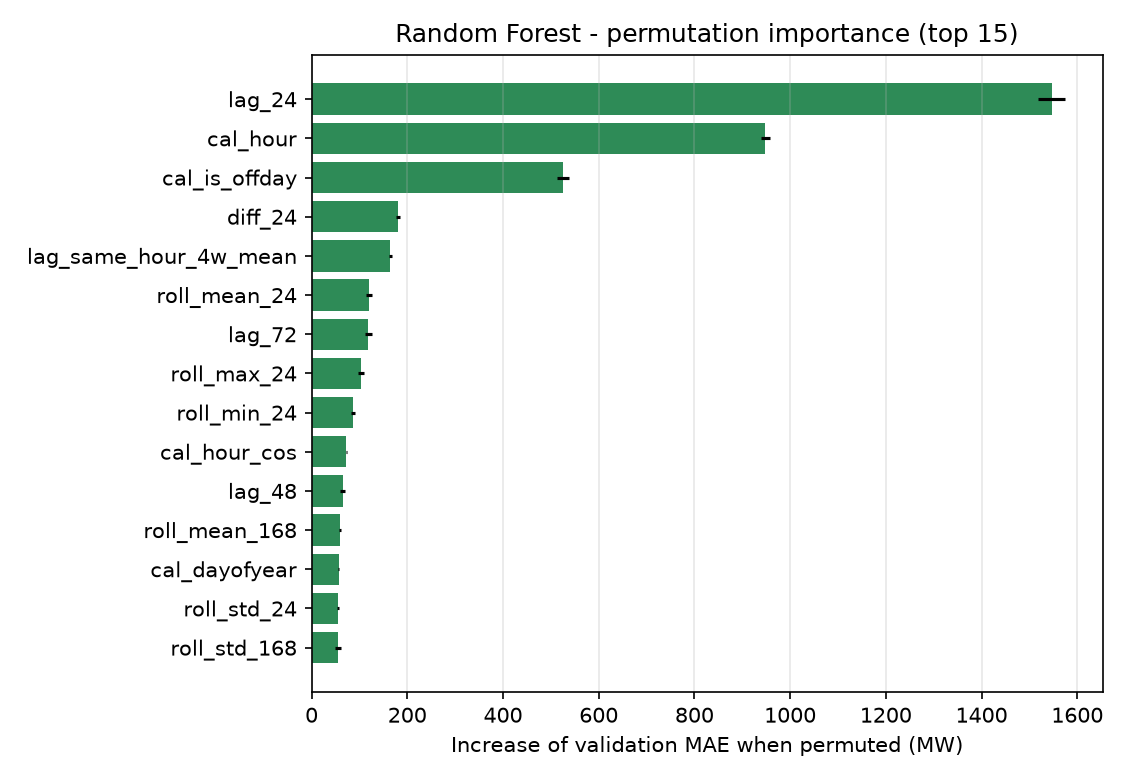
\includegraphics[width=0.8\linewidth]{b_feature_importance_rf.png}
\caption{Permutation importance (top 15) của Random Forest trên tập validation.}
\label{fig:perm-imp}
\end{figure}

Ba đặc trưng quan trọng nhất đến từ cả ba ý tưởng chính của phần B:
\code{lag_24} (+1\,546~MW khi bị xáo trộn), \code{cal_hour} (+948~MW) và \code{cal_is_offday} (+525~MW) ---
chính là biến ngày nghỉ tự xây dựng (cuối tuần \emph{hoặc} lễ). Tiếp theo là các đặc trưng lag phái sinh
(\code{diff_24}, \code{lag_same_hour_4w_mean}, \code{roll_mean_24}). Chỉ số impurity lại xếp \code{cal_hour}
cao nhất (0.45 so với 0.14 của \code{lag_24}), minh họa sự thiên vị nói trên.

\subsubsection{Ảnh hưởng của chân trời dự báo}\label{sec:horizon}

\begin{table}[H]
\centering
\caption{So sánh dự báo trước 1 giờ và trước 24 giờ (tập validation, cùng bộ đặc trưng và siêu tham số).}\label{tab:horizon}
\begin{tabular}{llrrr}
\toprule
Chân trời & Mô hình & MAE (MW) & RMSE (MW) & MAPE (\%)\\
\midrule
\multirow{3}{*}{$h=1$} & Ngây thơ $y_{t-1}$ & 1\,115 & 1\,507 & 3.91\\
 & Ridge & 405 & 677 & 1.42\\
 & Random Forest & \textbf{310} & \textbf{531} & \textbf{1.07}\\
\midrule
\multirow{3}{*}{$h=24$} & Ngây thơ $y_{t-24}$ & 2\,429 & 3\,507 & 8.43\\
 & Ridge & 1\,856 & 2\,513 & 6.39\\
 & Random Forest & \textbf{1\,536} & \textbf{2\,282} & \textbf{5.28}\\
\bottomrule
\end{tabular}
\end{table}

Khi được dùng $y_{t-1}$, mọi mô hình tốt hơn khoảng 5 lần. Điều này cho thấy hai điều: (i) chọn chân trời
là quyết định thiết kế quan trọng nhất và \textbf{phải được nêu rõ} khi so sánh với các kết quả khác --- nhiều
notebook công khai trên bộ dữ liệu này dùng lag 1 giờ nên có sai số thấp hơn nhiều; (ii) với $h=1$, Random
Forest đạt MAPE 1.07\%, xấp xỉ dự báo của TSO (1.05\%), gợi ý rằng dự báo TSO trong dữ liệu được cập nhật gần
thời gian thực chứ không phải dự báo ngày tới thuần túy (\cref{sec:baselines}).

\subsubsection{Một quan sát về chất lượng dữ liệu}\label{sec:data-quirk}

Khi phân tích sai số lớn nhất (\cref{sec:error-analysis}), phần B phát hiện chuỗi phụ tải có \textbf{tính mùa vụ
theo tuần yếu bất thường}: tự tương quan của phụ tải trung bình ngày ở độ trễ 7 ngày chỉ là 0.27 (nhỏ hơn
cả độ trễ 1 ngày, 0.37), và phụ tải trung bình Chủ Nhật chỉ thấp hơn Thứ Tư khoảng 12\%. Có những ngày cuối tuần
mang mức phụ tải của ngày làm việc (ví dụ Thứ Bảy 02/06/2018 trung bình 34\,328~MW, cao hơn mọi ngày trong
tuần trước đó) và ngược lại (Thứ Ba 05/06/2018 chỉ 23\,287~MW). Cột \code{total load forecast} của TSO cũng
bám đúng các bất thường này. Đây là đặc tính của dữ liệu nguồn chứ không phải lỗi của pipeline (các mốc thời
gian và tính liên tục theo giờ đã được kiểm tra), nhưng nó giới hạn độ chính xác mà các đặc trưng lịch có thể
mang lại. Nhóm đề xuất phần A kiểm tra thêm với dữ liệu gốc từ ENTSO-E/REE.

